\section{Discussion}
%
%\subsection{Reduction}
%As it as been mentioned in the introduction, the "abstraction reduction" does not always create smaller abstractions.
%This depends on the type of inputs (discrete, continuous), the number of dimension of inputs, the dimension of the suppressed subspace of the state space and the initial discretization of it.

\subsection{Covering/Overlap in the state space}
Ones should notes that the discretization of the state space in the case of the state extended abstraction might not have any equivalent with the same complexity (in term of number of symbols).
If we project the discretization on the original state space of the system,  the cells might overlaps.
We will see later that it can bring to improvement of the size of the abstraction in practice.

\begin{figure}
\centering
\begin{minipage}[b]{0.49\textwidth}
	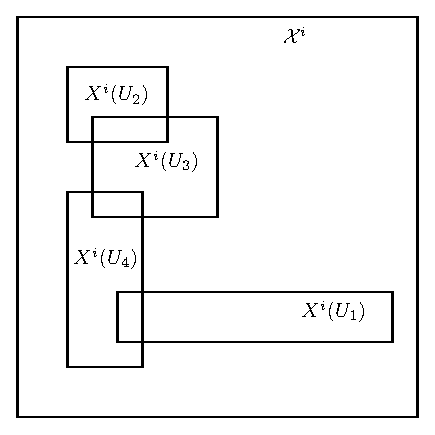
\includegraphics[width=\textwidth]{chapters/abstraction_reduction/overlapp_disc.eps}
\end{minipage}
\caption{The reached sets overlapps. The equivalent discretization of the state space on the left create an abstraction of 7 symbols for 4 symbols in the case of the input extended abstraction.}
\label{fig:overlapp}
\end{figure}

\subsection{Reachability}
Reachable sets are computed with the invariant set. As the invariant set is an over approximation of the state, this abstraction is not conservative. This means that for a given problem, it might exist a controller solution for the system $S'$ but no solution for the system $S_a$ (regardless of the memory number).

\section{Conclusion}
We have been creating an abstraction that is using input memories to replace the unobserved part of the state.
Experiments will show that this strategy might be interesting especially in case of systems with slow transient states (compared to the sampling time of the system).

The non observation of part of the state and the computation of the reachable sets in the linear monotone system case brought us to a bigger set of admissible noise sequences.
This will be particularly helpful to explain why this abstraction was more robust to mismodelling of the noise during experiments.

The size of the abstraction will depend on the number of memories and on the discretization of the state space and input space. These parameters are decided according to the given specifications. Therefore, it is not possible to infer when the extended abstraction might lead to more conservative abstraction than direct discretization of the state space.
Only simulations and experimentations on a specific problem will bring some results.

For most of the computation, the monotonic property has been used in order get analytical expressions.
It resulted in models that are really restrictive (any linear systems with non real eigenvalue is not monotonic). However, it was suitable in the case of the quadricopter.
Moreover, we have been choosing them mainly to simplify the computations. Ones should be able to extend this work easily to more complex models (by using numerical over approximation of the reachable set for example).